\section{Evaluating Overhead}
\label{sec:results}

In this section, we present the outcomes of our evaluation of \framework{},
focusing on its performance overhead in a real device while running various real
world apps.  We first quantify per API call overhead of \framework using
micro-benchmarks. And then evaluate memory and battery overhead of \framework{}
was evaluated using 10 most popular apps downloaded from the Google
Play Store.

All permissions requested by the apps were granted beforehand, and the apps were
subjected to 10 minutes of manual usage 5 times. All experiments were conducted
on a \textit{Samsung Galaxy M21} smartphone with a 2.3 GHz octa-core processor
and 4 GB of RAM running Android 12. 

% In this section, we present the outcomes of our evaluation of \framework{}, focusing on its practicality, compatibility, and performance against a variety of apps and configurations. We conducted extensive tests on the top 50 free apps available on the Android Play Store as of March 2, 2023, including 20 built-in apps provided with Stock Android and the two most popular banking apps on the Play Store. Additionally, we quantified microbenchmarks to measure the performance overhead of using \framework{} in different configurations, namely with \textit{LSPosed} without patching the APK and with \textit{LSPatch} by patching the APK.
% To quantitatively measure the microbenchmarks, we developed an in-house micro-benchmarking app that performed a consecutive series of API calls to retrieve user data. Throughout this process, we carefully monitored and recorded three key microbenchmark metrics: the time to execute these API calls, the amount of RAM consumed, 
% % the CPU overhead incurred, 
% and the impact on battery drainage during the experimental trials.
% % To assess the app's feasibility and compatibility, we conducted hands-on testing across four different configurations involving patching and spoofing the user data of various apps. The results were meticulously recorded through manual observations. However, to quantitatively measure the microbenchmarks, we developed a specialized application that performed a consecutive series of 1000 API calls to retrieve user data. Throughout this process, we carefully monitored and recorded four key microbenchmark metrics: the time to execute these API calls 1000 times, the amount of RAM consumed, the CPU overhead incurred, and the impact on battery life during the experimental trials.
% % \subsection{Micro-benchmarking Performance Overhead}
% % \subsection{Performance Overhead}
% % To assess the performance impact of the \framework{}, we conducted a series of experiments using a benchmarking app for evaluating time elapsed overhead. 
% The benchmarking app was remotely executed 100 times using Python scripts and the \textit{Wifi\_ADB} tool. We aimed to evaluate the app's performance across two different configurations: Without Spoofing (for a baseline) and With Spoofing. We configured the micro-benchmarking app for each permission to call popular API methods that retrieve user data. 
% To ensure consistent results throughout the experiments, we applied the deception policies  in Table \ref{tab:benchmarking_strategy} within the \framework{} framework.

%This setup provided a suitable environment for assessing \framework{}'s performance overhead.

% \begin{table}[htbp]
    \caption{Benchmarking and Deceiving Strategy used for each permission while evaluating performance overhead }
    {\tiny
    \begin{center}
        % \begin{threeparttable}
            \begin{tabular}{|>{\centering}m{0.15\linewidth}|m{0.4\linewidth}|m{0.26\linewidth}|}
                \hline
                \textbf{Permission} & \textbf{\textit{Bench-marking Strategy}} & \textbf{\textit{Deceived by}} \\
                \hline
                Calendar & Calls \texttt{ContentProvider. query()} for calendar events and traverse. & a database cursor with 30 fake calendar events rows.\\
                \hline
                Call Log & Calls \texttt{ContentProvider. query()} API for call logs and traverse. & a cursor to the database with 30 fake call logs. \\
                \hline
                Camera & Display the camera stream preview frame using \texttt{camera2} API. & the preview frame with a black image of same resolution. \\
                \hline
                Clipboard & Sets text of a \texttt{textView} with \texttt{ClipboardManager.prim- aryClip} text & a random string generated of arbitrary size.  \\
                \hline
                Contacts & Calls \texttt{ContentProvider. query()} API for contacts and traverse. & a cursor to the database with 30 fake contacts. \\
                \hline
                Location & Calls \texttt{LocationManager. getLastKnownLocation()} and logs the lats and longs & randomly generated float values  for lats and longs\\
                \hline
                Messages & Calls \texttt{ContentProvider. query()} API for messages and traverse. & a cursor to the database with 30 fake messages. \\
                \hline
                Network & \texttt{WifiManager.getConnec- tionInfo()} is called to log information like SSID. & randomly generated strings of arbitrary size. \\
                \hline
                Packages &  Calls \texttt{PackageManager. getInstalledPackages()} API and traverses over the list. & a list of 25 deceived packages \texttt{PackageInfo}. \\
                \hline
                Tracking & Logs various information fetched using \texttt{Telephony- Manager.getString()}. & randomly generated strings satisfying the patterns.  \\
                \hline
            \end{tabular}
            % \begin{tablenotes}
            %     \item[1] To maintain the consistency before and after deceiving the permission, the number of rows in the cursor returned by the \texttt{query()} method was maintained to be 30.
            %     \item[2] To maintain the consistency before and after deceiving the permission, after deceiving the permission, \framework{} was modified to return the first 25 packages as deceived and the rest as returned by the non-hooked method call.
            % \end{tablenotes}
        %  \end{threeparttable}
    \end{center}
    }
    \label{tab:benchmarking_strategy}
\end{table}

% \subsubsection{CPU Utilization}
% To evaluate the average CPU usage of a process, we rely on data stored in the \texttt{/proc/self/stat} file and calculated the average CPU usage percentage using the following equation:

% % , which serves as a comprehensive source of process status information in the kernel source file. 

% % This file provides the necessary metrics for assessing CPU usage, including (a) User mode process time ($u_{time}$), (b) Kernel mode process time ($k_{time}$), (c) User mode waiting time for child processes ($uw_{time}$), (d) Kernel mode waiting time for child processes ($kw_{time}$), and (e) Start time of the process ($s_{time}$). All measurements obtained from the status file are expressed in clock ticks.

% \begin{figure}[t]
% 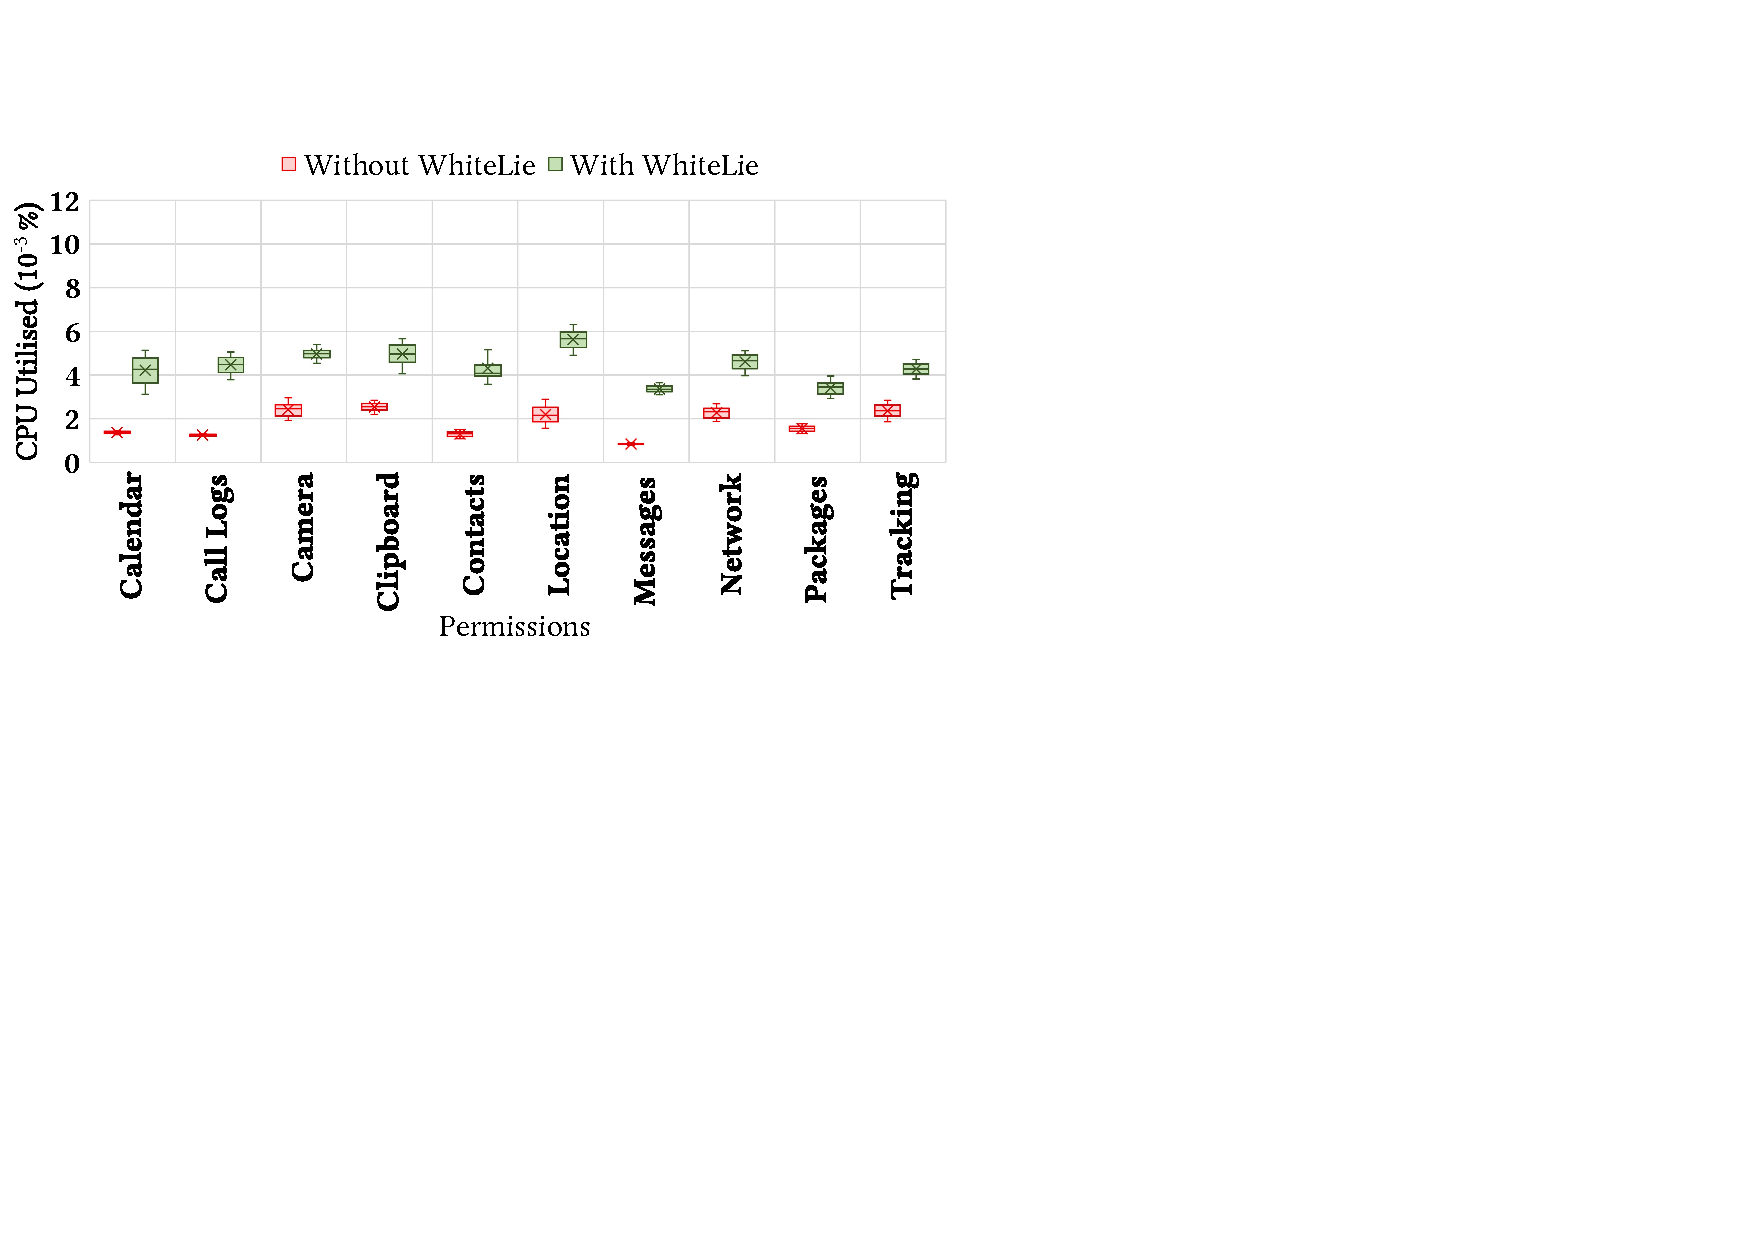
\includegraphics[width=\linewidth]{figures/performance_overhead/results_cpu_utilized.pdf}
% \caption{CPU Utilisation performance overhead for various Permissions in different configurations}
% \label{fig:reslts_cpuUsed}
% \end{figure}

% % In order to calculate the average CPU usage, information about the number of cores and their clock speed are required which can be accessed via \texttt{android.system.OsConstants} class. The number of cores ($numCores$) and clock speed in Hertz ($clockSpeed$) can be retrieved using the \texttt{\_SC\_NPROCESSORS\_CONF} and \texttt{\_SC\_CLK\_TCK} constants from \texttt{OsConstants} respectively. 
% % Additionally, the device's uptime ($upTime$), which represents the elapsed time since boot, can be obtained using the \texttt{SystemClock.elapsedRealtime()} method, returning the value in milliseconds.

% $$avgUsagePercent =  \frac{cpuTime}{processTime * numCores} * 100$$

% where, $$cpuTime = \frac{u_{time} + k_{time} + uw_{time} + kw_{time}}{clockSpeedHz}$$

% and, $$processTime = \frac{upTime}{1000} - \frac{s_{time}}{clockSpeed}$$

% % To assess the impact of the \framework{} on CPU usage in the target app across different configurations, we obtained the status of the target app process by accessing the \texttt{/proc/self/stat} file. 
% % We used the abovementioned formula to calculate the Average CPU Usage Percentage and logged the results. 
% Figure \ref{fig:reslts_cpuUsed} illustrates the data extracted from the log file. Across various permissions in both configurations, the target app experiences an average CPU usage overhead of \textbf{0.000143\%}. It is important to note that this overhead is negligible and arises from the operations executed by the hooks, which gather user policy information to deceive the results of the hooked API method.

\subsubsection*{\textbf{API call overhead}} 
We measure the time elapsed during code execution by executing hooked
API methods within the \texttt{Timing.measureNanoTime()} method.
% , and recording the returned values to a log file.
% To measure the time elapsed during code execution, we utilised the \texttt{Timing.measureNanoTime()} method. This method takes a code block as input and returns the elapsed time in nanoseconds. We recorded the returned values in a log file by executing the respective API methods within the \texttt{measureNanoTime()} method. 
% \begin{figure}[t]
% 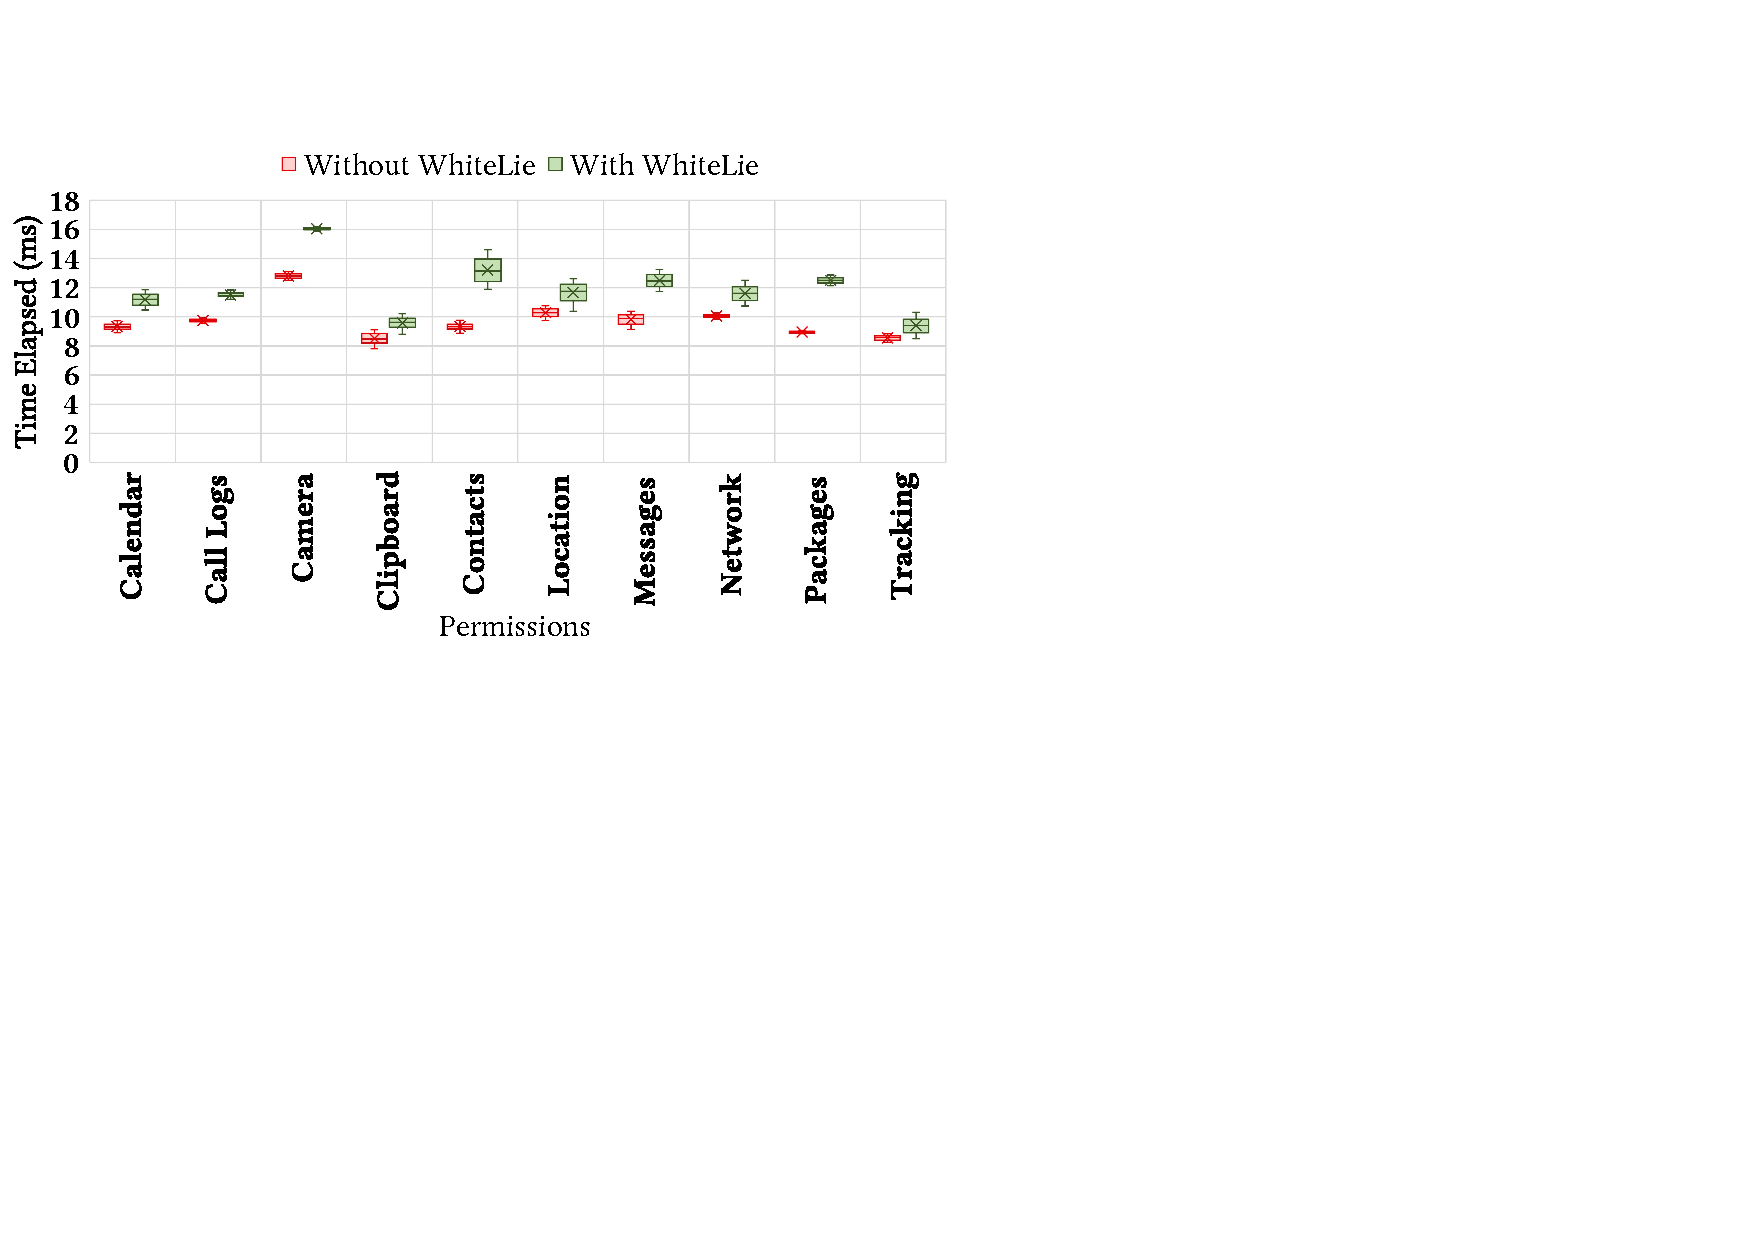
\includegraphics[width=\linewidth]{figures/performance_overhead/results_time_elapsed.pdf}
% \caption{Time elapsed for fetching user data for various Permissions in different configurations}
% \label{fig:reslts_timeElpsd}
% \end{figure}
% Figure \ref{fig:reslts_timeElpsd} displays the time logs captured by the target app, showcasing the time taken to fetch resource data for various permissions in different configurations. 
We observed an average overhead of 1.64 ms across different API calls.
The increase in elapsed time is because of the operations performed by the
hooks. For user data like contacts and camera, we experienced an overhead of
3.87 ms and 3.23 ms respectively. For tracking and clipboard user data, we
observed an overhead of 0.83 ms and 1.07 ms respectively. The overhead depends
on the operations performed by the respective permission-deceiving hooks. For
contacts and camera APIs, we are performing intensive operations like reading a
database and manipulating pixels of an image, whereas for tracking and clipboard
APIs, we are simply returning a deceived string.

Many of these APIs were called several times during the app runs in our
experiments as shown in Figure~\ref{fig:reslts_noAPICalls}. The API call
overhead, however, did not impact the performance of the apps we tested in any
observable manner.

\begin{figure}[t]
    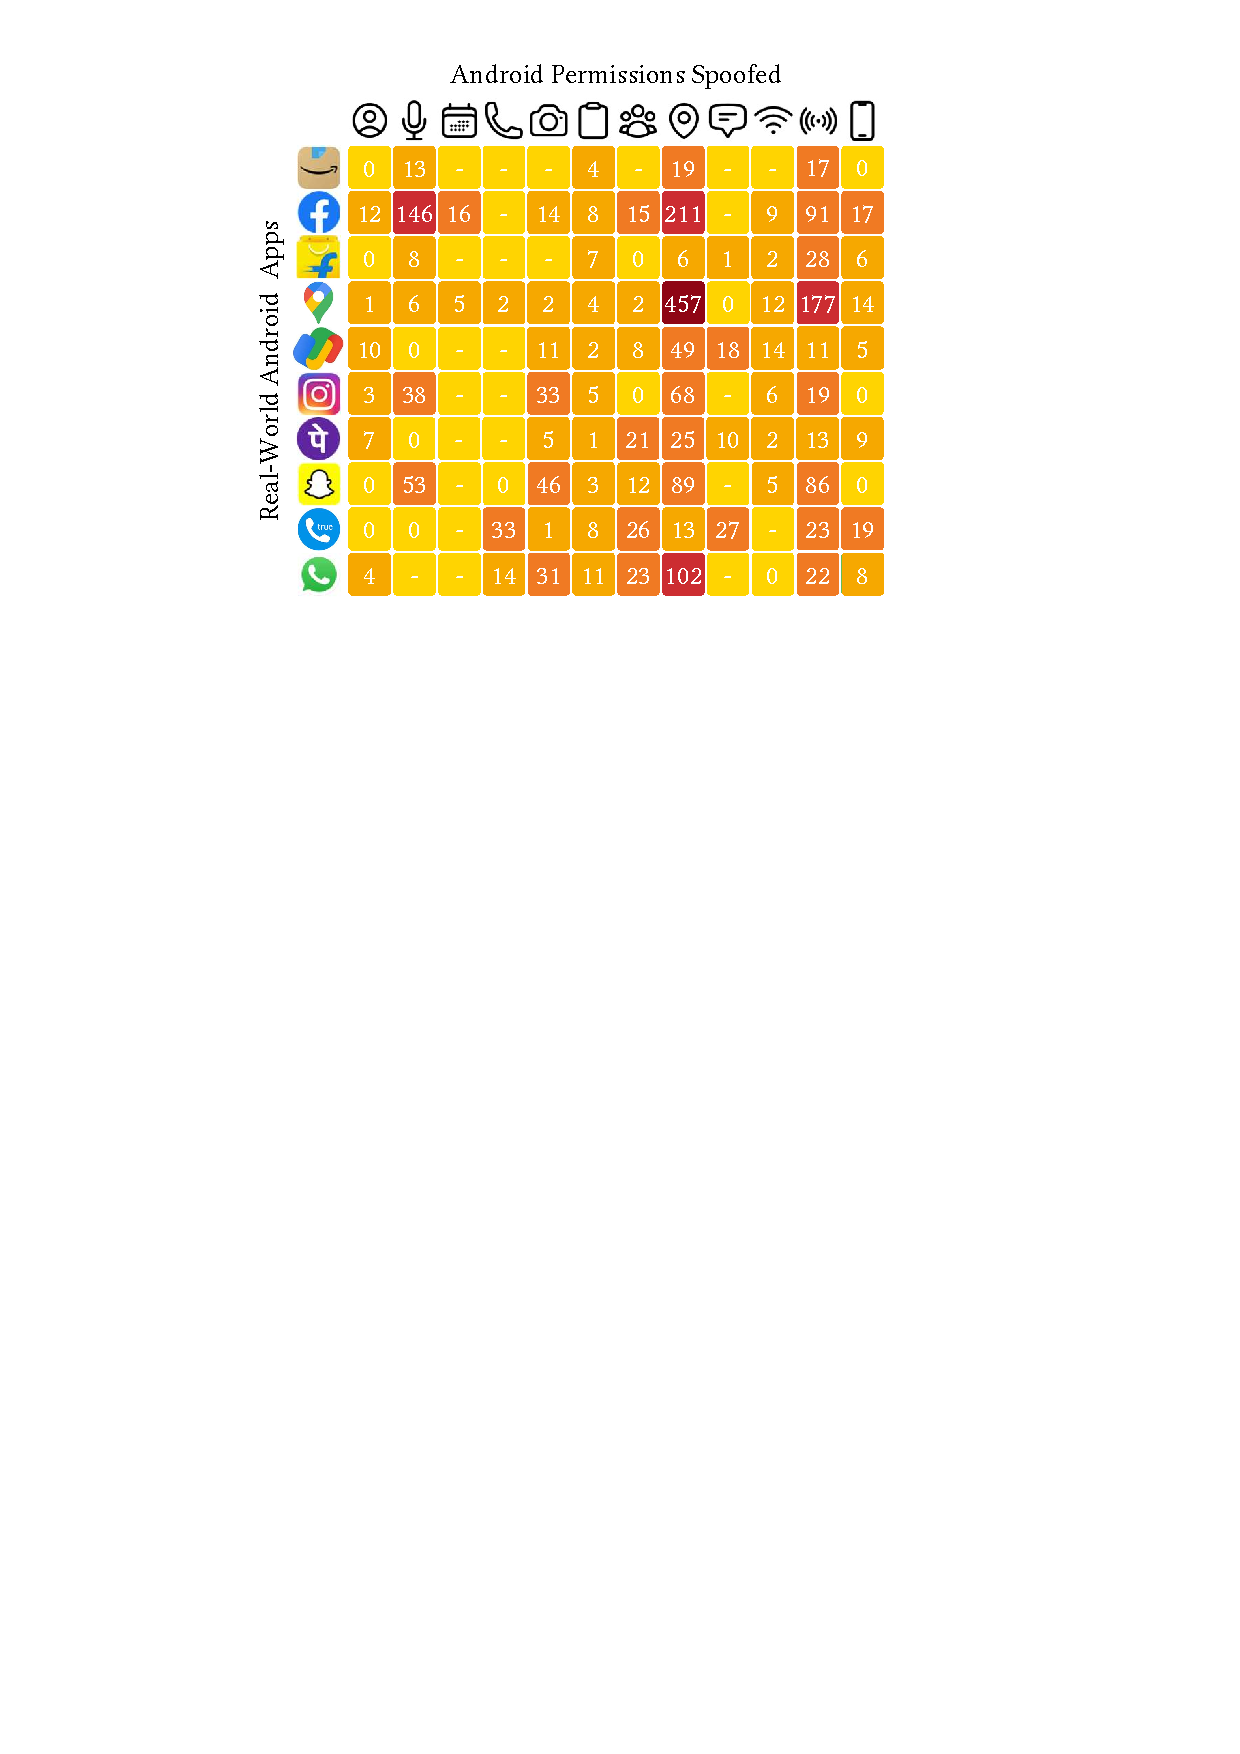
\includegraphics[width=0.8\linewidth]{Figures/Performance Evaluation/evaluation_api_calls_heatmap.pdf}
    \caption{Heatmap illustrating number of API calls made by various popular apps while evaluating performance overhead.}
    \label{fig:reslts_noAPICalls}
\end{figure}

% , which are relatively simple and do not significantly impact the duration of user data retrieval.
% This demonstrates that users can expect prompt execution of their target apps while utilising \framework{} to safeguard their privacy. 
\subsubsection*{\textbf{Memory Used}} 
The memory utilization of the benchmarking app was measured using \textit{ADB}'s
\textit{dumpsys} tool, using the \textit{Proportional Set Size (PSS)} metric.
This metric captures the shared memory proportionally used by each
process.

% The memory utilisation of the target app, \framework{}, patcher, and system was measured using \textit{ADB}'s \texttt{dumpsys} tool, using the \textit{Proportional Set Size (PSS)} metric. This metric accurately captures the shared memory proportionally used by each process. \ref{sec:appendixA} presents detailed information on individual memory usage for the different processes. 

\begin{figure}[t]
    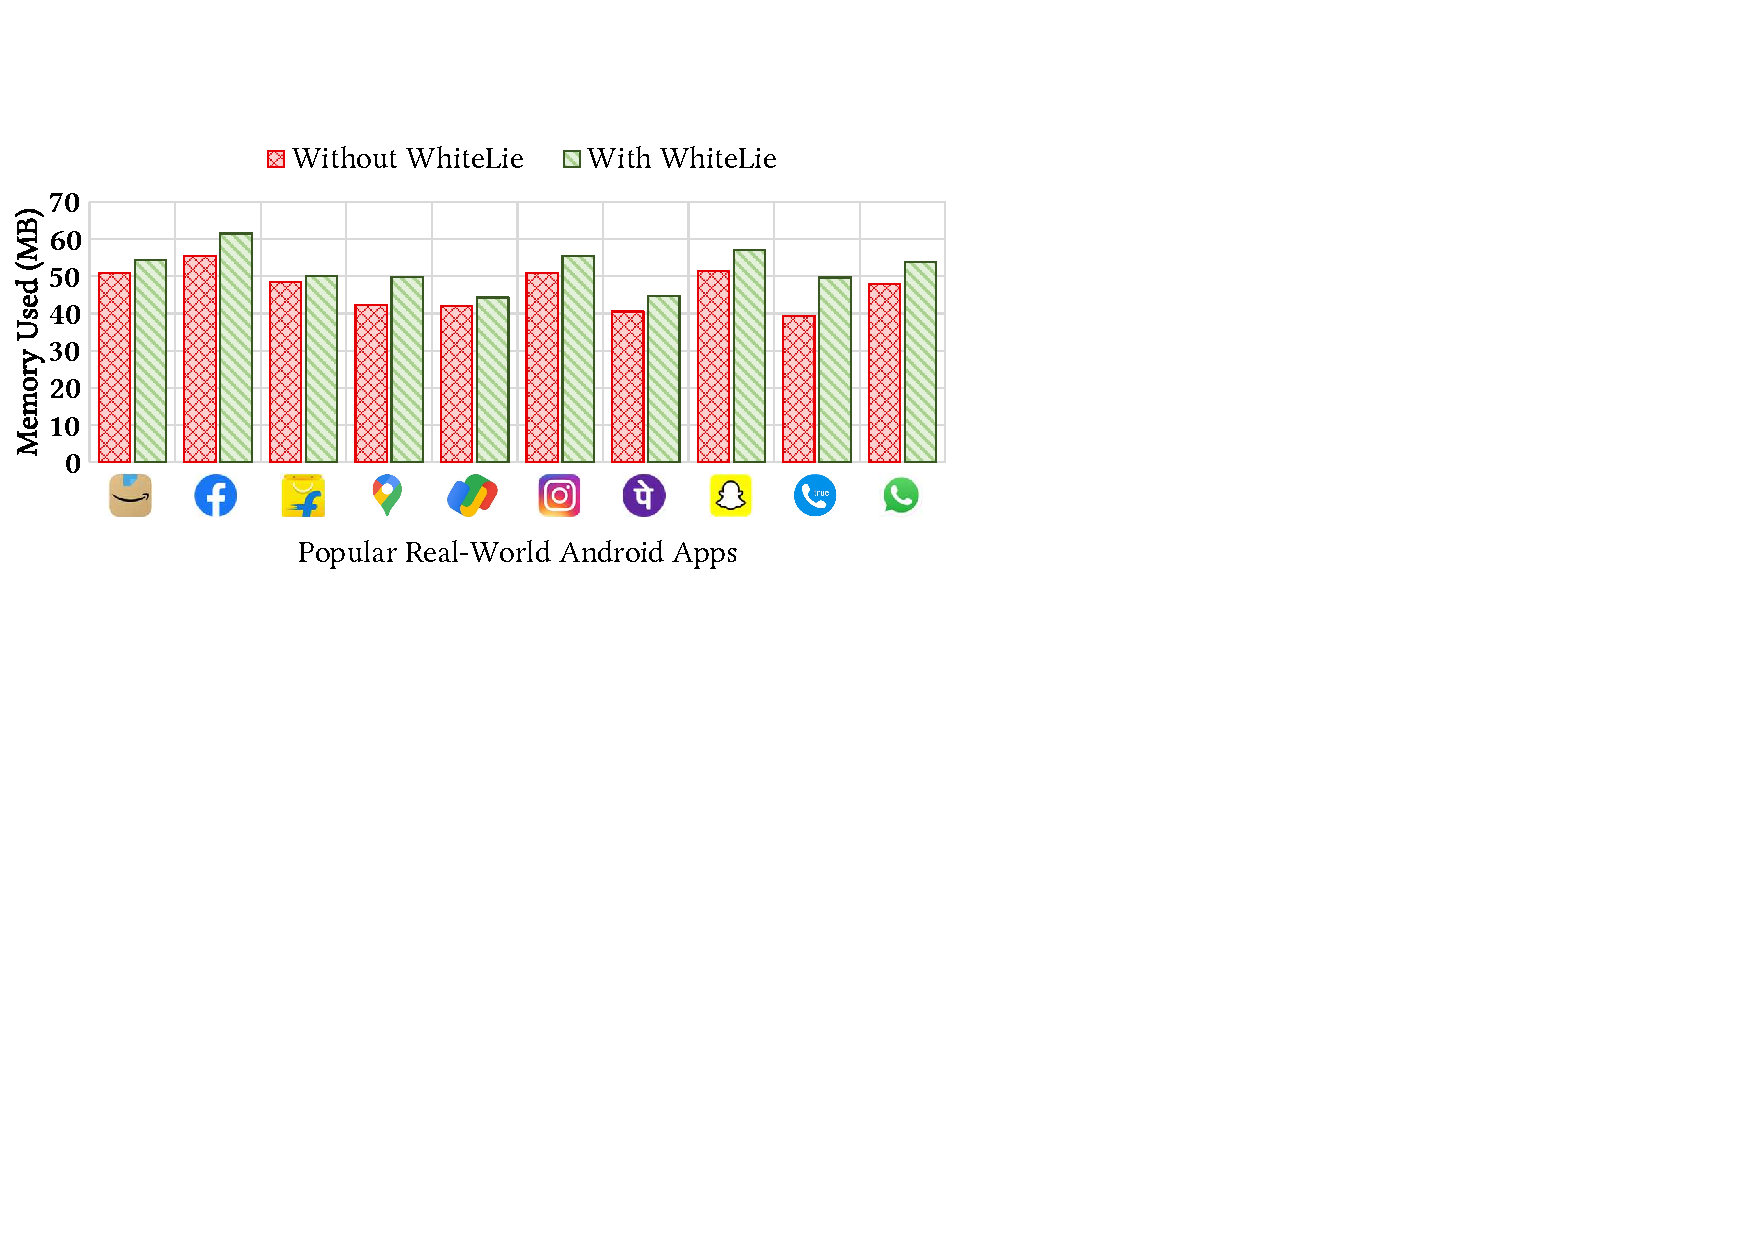
\includegraphics[width=\linewidth]{Figures/Performance Evaluation/results_memory_used_target_app_real_world_apps.pdf}
    \caption{Memory used by various Android apps with and without \framework{}.}
    \label{fig:results_memUsedAll}
\end{figure}

% The experimental results demonstrate that \framework{} and the patcher exhibit consistent memory usage without significant overhead across different configurations. This outcome is reasonable since both processes perform similar operations in each configuration.

% When utilising \framework{} in both configurations, the system process experiences an expected average memory overhead of \textbf{4.87 MB} across all permissions. This minimal overhead can be attributed to the system process's involvement in process creation, which remains consistent across scenarios. Similarly, when employing the patcher, the system process encounters a negligible average overhead of \textbf{5.58 MB} across all permissions.

% However, the target app bears the brunt of memory overhead in various configurations. 

Figure~\ref{fig:results_memUsedAll} shows that the memory overhead while using
\framework{} on various real-world apps is negligible.  On average, \framework
only incurs 5.2 MB of memory overhead. 
% The additional
% memory usage is justifiable considering the target app's execution of extra
% lines of code and instructions during the retrieval of resource data due to the
% hooking process. The hooking method involves utilizing the query method to
% evaluate user-defined policies and applying the necessary hooks accordingly.

% Notably, the memory overhead experienced by the target app varies among different permissions, as each permission involves distinct operations during hooking, leading to varying overhead levels. Permissions like Clipboard and Location exhibit negligible average memory overhead of 3.42 MB, as they involve relatively straightforward operations. In contrast, permissions like Camera and Call Logs experience an average memory overhead of 6.62 MB due to their more complex operations.

\subsubsection*{\textbf{Battery Discharged}} 
To accurately measure the device's battery usage during our experiments, we
utilized the \textit{ADB}'s \textit{batterystats} tool~\cite{batterystats}.
Before each experiment, we ensured a clean slate by resetting the tool. To
mitigate any potential inconsistencies in battery usage statistics, we remotely
connected the device via \textit{Wifi ADB}, as physically connecting it to a PC
can inadvertently charge the device and yield inaccurate results. 
% Additionally, we disabled Bluetooth and phone data connection to maintain a
% consistent testing environment. 
By leveraging \texttt{batterystats}'s \textit{discharge} metric, we could
quantify the amount of battery discharged since the last charge, accounting for
the impact by both the target app and the system. 
% It is worth noting that the battery status evaluation methods consume minimal energy compared to other components like the display.

\begin{figure}[t]
    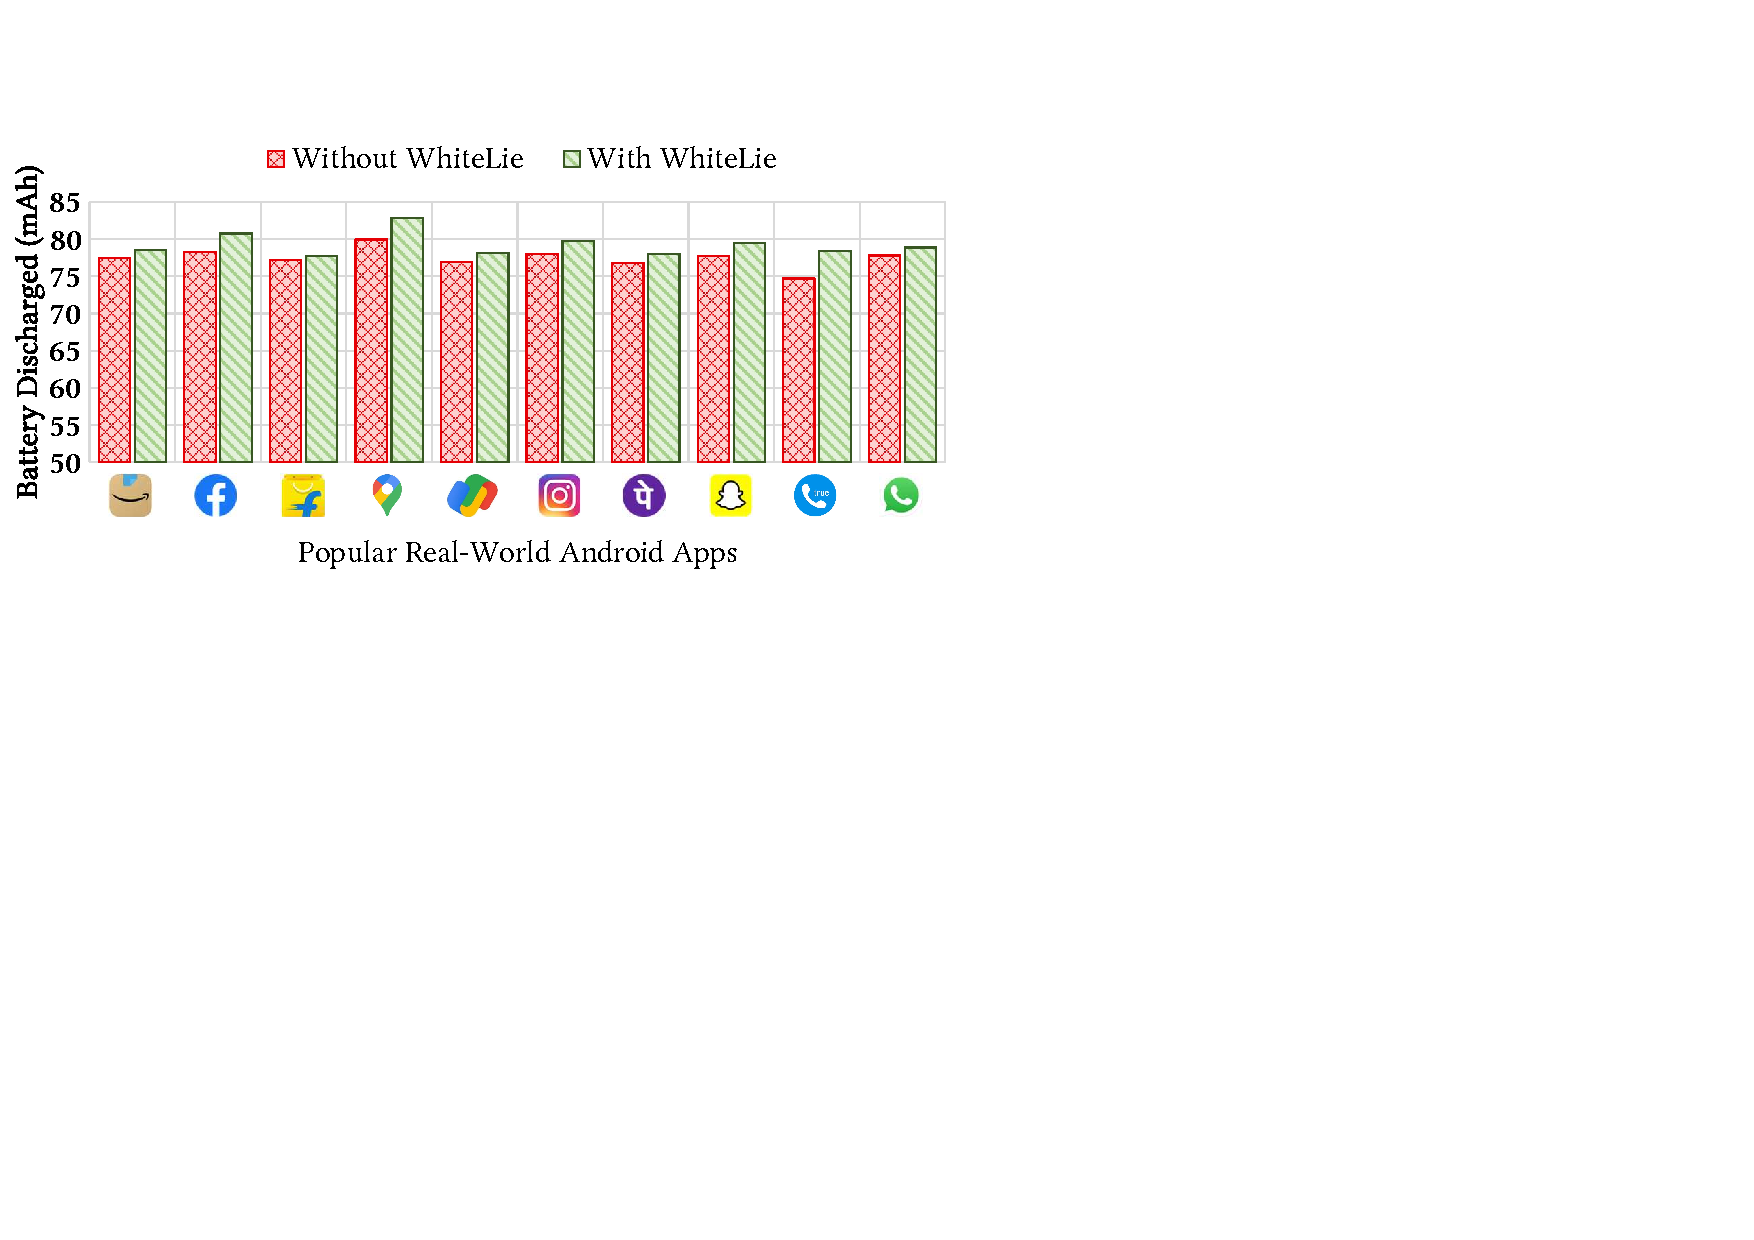
\includegraphics[width=\linewidth]{Figures/Performance Evaluation/results_battery_discharged_real_world_apps.pdf}
    \caption{Battery discharged by various Android apps with and without \framework{}.}
    \label{fig:reslts_btryDschrgd}
\end{figure}

% However, we must acknowledge that we observed significant variations in the results due to the involvement of various unaccounted processes and parameters. 
Figure \ref{fig:reslts_btryDschrgd} shows the battery drained during the 
app runs with and without \framework. It shows that \framework's impact on
battery drain is negligible. An average additional discharge of approximately
1.76 mAh (2.52\%) was observed across the 5 minute runs of various apps experimented when
they were run with \framework. 

\textit{Overall, our experiments show that \framework's usage has a minimal impact on
app's performance, app's memory consumption, and the device's battery drain. 
This shows that \framework is a versatile and efficient approach to protecting
user privacy.}

We further experimented with actively reducing battery drain using \framework{}.
In particular, by returning \texttt{null} from the
\texttt{beforeHookedMethod()}, the method calls to the original method can be
blocked which can save battery consumed by sensors and other components. To 
examine this, we added a battery saver mode to \framework{} that selectively
blocks Android API calls according to user policies. 
To quantitatively measure the battery drainage, we developed a benchmarking app that performed a consecutive series of 1000 API calls to retrieve user data.
We observed this approach can save an average of 4.08 $\mu{}Ah$
(60.83\%) per API call.


\begin{figure}[t]
    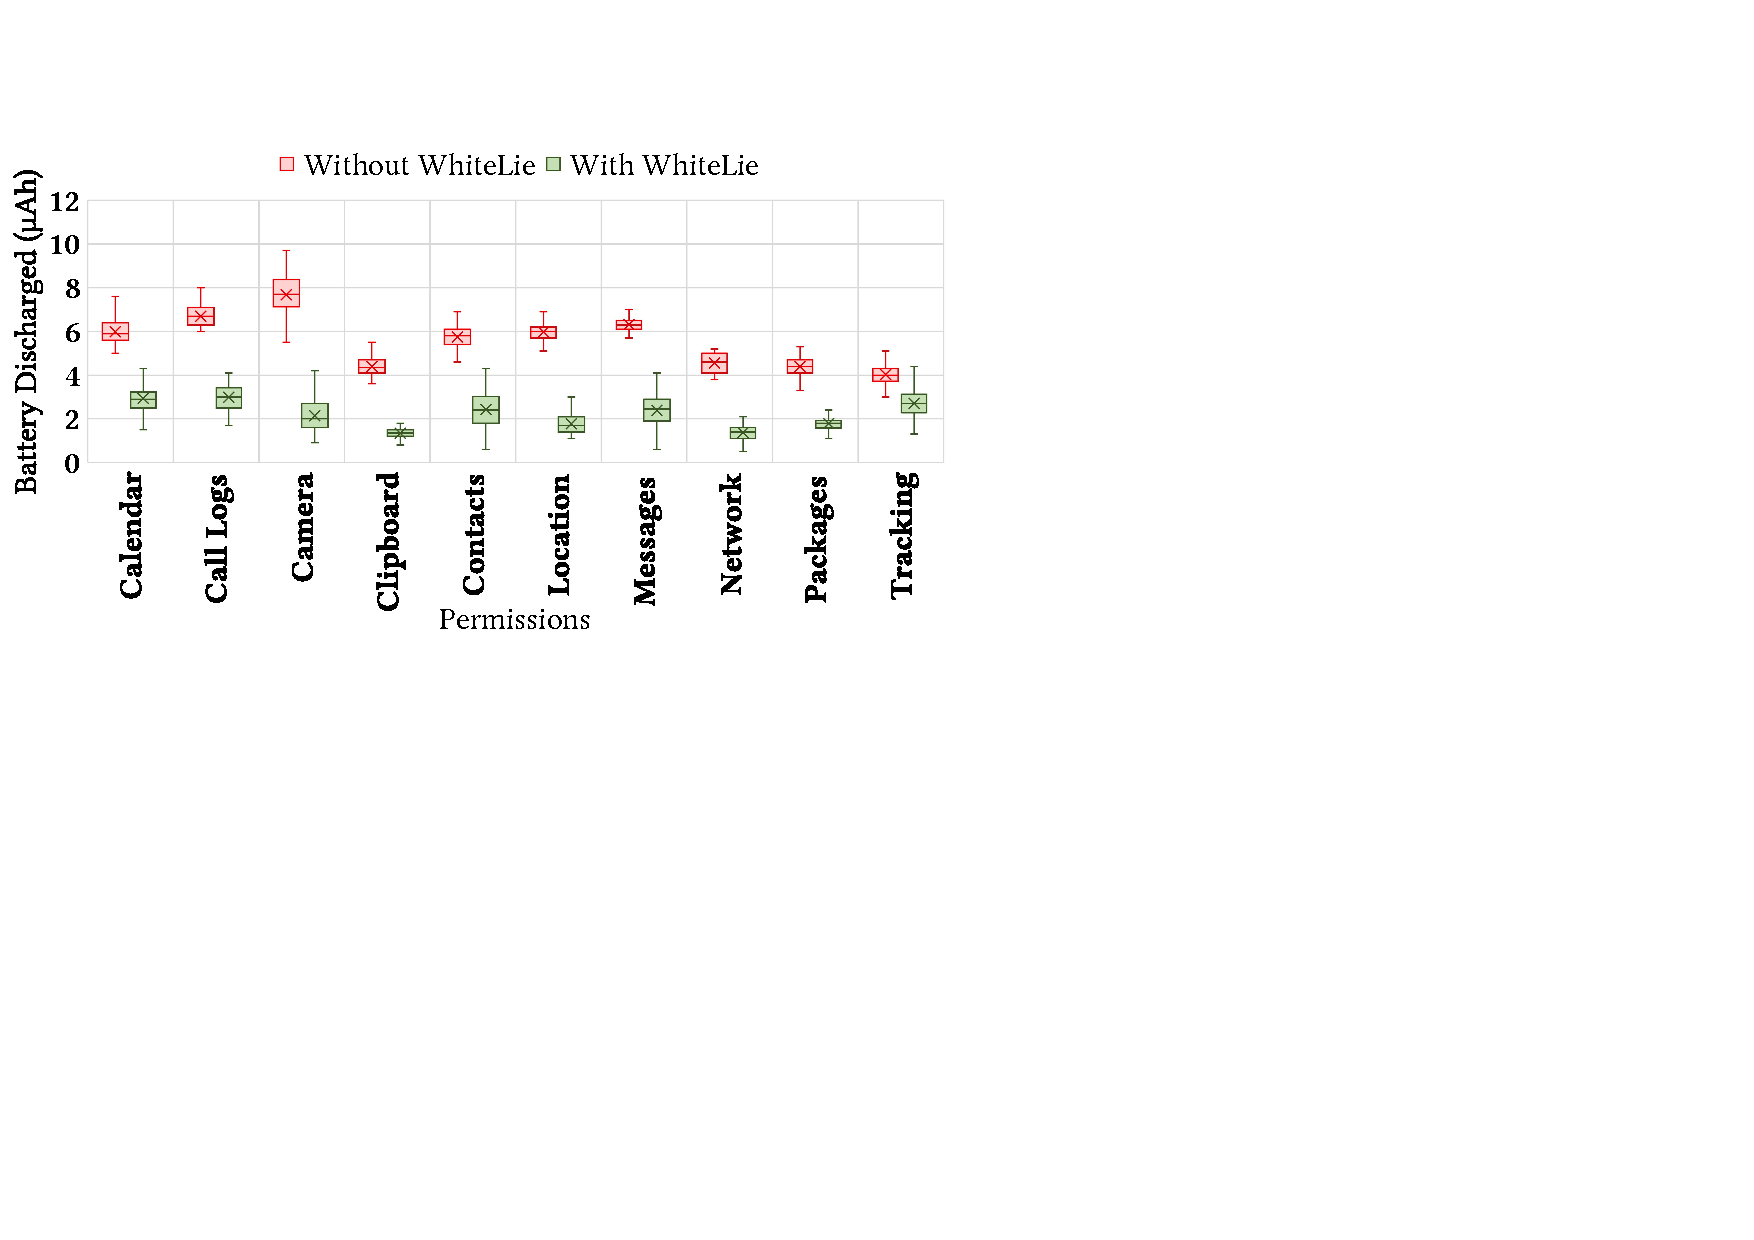
\includegraphics[width=\linewidth]{Figures/Performance Evaluation/results_battery_discharged_battery_saver.pdf}
    \caption{Battery discharged by benchmarking app while fetching user data for various Permissions with and without \framework{}.}
    \label{fig:reslts_btrySaver}
\end{figure}


% \framework{} can also block apps from receiving user data altogether. By blocking user data, \framework{} can prevent Android APIs from being called, resulting in reduced battery consumption. Listing \ref{lst:btrySvr} explains the approach employed to block sensitive APIs from being called at the first place by returning \texttt{null} from the \texttt{beforeHookedMethod()} and ultimately saving battery. \framework{} offers customisable battery saver that selectively blocks Android API calls according to user, conserving battery usage by sensors, processor, and other components. Figure \ref{fig:discus_btrySavr} illustrates the results of the battery saver feature, showing an average of \textbf{4.08 mAh} amount of battery drainage saved across all permissions.

% \begin{lstlisting}[caption={Kotlin code to save battery by returning \texttt{null} based on \texttt{batterySaver} policy defined by user},label={lst:btrySvr},language=Kotlin]
override fun beforeHookedMethod(_:MethodHookParam){
    val cursor = getDeceitSettings() 
    val bs = getString(cursor, "batterySaver")
    if(bs == "true") return null
    cursor.close()
}
\end{lstlisting}